\section{A concave cometric and smooth product cores}
\label{sec:cometric}

We construct the metric in two stages.  First we join the two product
structures by a metric on the torus neck.  Then we extend its endpoint
formulas over compact punctured-torus products.  The neck estimates will
depend on a small parameter $\delta$, while the torus periods will be
chosen afterward to fit the surface boundaries into hyperbolic cusps.

\subsection{The matrix path and its endpoint coordinates}

Write $e_1,e_2$ for the standard basis of $\mathbb R^2$.
The two product structures require different diagonal coordinate frames:
$(e_1,e_2)$ on the left and $(e_2+\epsilon e_1,e_1)$ on the right.
To arrange concavity, we start with a diagonal path and introduce the
shear only where both diagonal coefficients have strictly negative
second derivative.  The diagonal variation has size $\delta$;
taking $\epsilon=\delta^2$ makes the frame change a smaller perturbation.
The periods $B_1=\epsilon B_2$ then turn this small coordinate shear into
the fixed integral gluing of Section~\ref{sec:topology}.

Define the
smooth function $a:\mathbb R\to[0,1)$ and its primitive $A$ by
\begin{equation}\label{eq:cometric-cutoff}
 a(u)=\begin{cases}
       \exp\bigl(-1/(2/3-u)\bigr),&u<2/3,\\
       0,&u\ge 2/3,
      \end{cases}
 \qquad A(u)=\int_0^u a(y)\,dy.
\end{equation}
The definition includes negative $u$, which will be needed when extending
the metric into the product pieces.  Fix once and for all a smooth
nondecreasing function $\chi:\mathbb R\to[0,1]$ equal to zero on
$(-\infty,5/12]$ and to one on $[7/12,\infty)$.
For $0<\delta\le 1/2$, set $\epsilon=\delta^2$ and define
\begin{align}
 H(t)&=e_2+\epsilon\chi(t)e_1,\notag\\
 d_1(t)&=1+\delta A(t),\qquad
 d_2(t)=1+\delta A(1-t),\notag\\
 P(t)&=d_1(t)e_1e_1^{\mathsf T}+d_2(t)H(t)H(t)^{\mathsf T},
 \qquad 0\le t\le1.
 \label{eq:cometric-path}
\end{align}
Here a superscript $\mathsf T$ denotes transpose.  For a positive definite
matrix $P$, its inverse $Q=P^{-1}$ is the matrix of the torus metric;
we therefore call $P$ the cometric.

Choose $B_2>0$ later and put $B_1=\epsilon B_2$.  On
\[
 T^2=\mathbb R^2/\Lambda,\qquad
 \Lambda=\mathbb Z B_1e_1+\mathbb Z B_2e_2,
\]
use the neck metric
\begin{equation}\label{eq:neck-metric}
 g=dt^2+dx^{\mathsf T}Q(t)\,dx.
\end{equation}
The product coordinates at the two ends are given by the frames
\begin{equation}\label{eq:end-frames}
 T_1=(e_1,e_2),\qquad T_2=(e_2+\epsilon e_1,e_1),\qquad x=T_i y.
\end{equation}
At the first end the two coordinate periods are $B_1,B_2$; at the second
they are $B_2,B_1$. The first coordinate is the surface-boundary direction
and the second is the circle factor. The period calculation
\eqref{eq:torus-periods} shows that these frames give exactly the gluing
\eqref{eq:torus-gluing}.

Let $\tau=t$ at the first end and $\tau=1-t$ at the second, so that
$\tau$ increases into the neck.  A constant coordinate change $x=T_i y$
changes the cometric by $P\mapsto T_i^{-1}PT_i^{-\mathsf T}$.
Since $A$ is constant on $[2/3,\infty)$, in these endpoint coordinates
we have the exact identities
\begin{equation}\label{eq:end-cometric}
 P_i(\tau)=\begin{pmatrix}1+\delta A(\tau)&0\\0&b\end{pmatrix},
 \qquad b=1+\delta A(1),\qquad 0\le\tau\le1/4.
\end{equation}
In particular
\begin{equation}\label{eq:end-cometric-slope}
 P_i(0)e_1=e_1,
 \qquad P_i'(0)=\kappa e_1e_1^{\mathsf T},
 \qquad \kappa=\delta a(0)>0.
\end{equation}
Primes on $P_i$ refer to $\tau$.

For symmetric matrices $R,S$, write $R\preceq S$ when $S-R$ is
positive semidefinite; $R\succeq S$ has the reversed meaning.

\begin{lemma}\label{lem:cometric-bounds}
There are constants $\delta_0>0$ and $C<\infty$, depending only on the
fixed function $\chi$, such that for $0<\delta\le\delta_0$ the path
\eqref{eq:cometric-path} satisfies, in the original coordinates and in
either endpoint coordinate system,
\begin{gather}
 \frac19\operatorname{Id}\preceq P\preceq18\operatorname{Id},
 \qquad
 \frac1{18}\operatorname{Id}\preceq Q\preceq9\operatorname{Id},
 \qquad \|P'\|\le C\delta,
 \label{eq:cometric-uniform}\\
 -P''\succeq0,
 \qquad |P'p|^2\le C\delta\,p^{\mathsf T}(-P'')p
 \quad\text{for every }p\in\mathbb R^2.
 \label{eq:cometric-domination}
\end{gather}
The constants do not depend on $B_1$ or $B_2$.
\end{lemma}

\begin{proof}
All matrix norms are Euclidean operator norms.
On $[0,1]$ we have $1\le d_i\le2$.  The matrix
$R=(e_1,H)$ and its inverse have squared norms at most $3$.
As $P=R\operatorname{diag}(d_1,d_2)R^{\mathsf T}$, this gives
$\operatorname{Id}/3\preceq P\preceq6\operatorname{Id}$ in the original
coordinates.  The same bounds on $\|T_i\|^2$ and $\|T_i^{-1}\|^2$
give the displayed weaker bounds in both endpoint frames.

For $u<2/3$,
\begin{equation}\label{eq:cutoff-differential}
 a'(u)=-\frac{a(u)}{(2/3-u)^2}.
\end{equation}
Consequently, on $[0,1]$,
$a^2\le-a'$ and $|a'|\le1$, with both sides zero on the plateau when
appropriate.  Put $I_0=[5/12,7/12]$.
Outside $I_0$, the vector $H$ is constant.  If $q=R^{\mathsf T}p$,
then
\[
 p^{\mathsf T}(-P'')p
 =\delta\bigl(-a'(t)q_1^2-a'(1-t)q_2^2\bigr),
\]
and
\[
 |P'p|^2
 \le3\delta^2\bigl(a(t)^2q_1^2+a(1-t)^2q_2^2\bigr)
 \le3\delta\,p^{\mathsf T}(-P'')p.
\]
This proves concavity and the required domination there, including the
directions in which $-P''$ vanishes.

On $I_0$ both $t$ and $1-t$ lie in $[5/12,7/12]$, and
\[
 -a'(t),\ -a'(1-t)\ge m,\qquad m=144e^{-12}>0.
\]
To control every error caused by the moving frame, compare $P$ with
$P_0=\operatorname{diag}(d_1,d_2)$ and write $E=P-P_0$.
The derivatives are
\begin{align*}
 P'={}&\delta a(t)e_1e_1^{\mathsf T}
       -\delta a(1-t)HH^{\mathsf T}
       +d_2\epsilon\chi'(e_1H^{\mathsf T}+He_1^{\mathsf T}),\\
 P''={}&\delta a'(t)e_1e_1^{\mathsf T}
       +\delta a'(1-t)HH^{\mathsf T}
       -2\delta a(1-t)\epsilon\chi'
              (e_1H^{\mathsf T}+He_1^{\mathsf T})\\
       &+d_2\epsilon\chi''(e_1H^{\mathsf T}+He_1^{\mathsf T})
       +2d_2\epsilon^2(\chi')^2e_1e_1^{\mathsf T}.
\end{align*}
Using $|H|\le\sqrt2$ and
$\|HH^{\mathsf T}-e_2e_2^{\mathsf T}\|\le3\epsilon$ gives
\[
 \|E'\|\le C_1\epsilon,
 \qquad \|E''\|\le C_2\epsilon,
\]
where $C_1,C_2$ depend only on the fixed function $\chi$.
These estimates use only $\delta,\epsilon\le1$ and $d_2\le2$.
Take
$\delta_0\le\min\{1/2,m/(2C_2)\}$.
Since $\epsilon=\delta^2$ and $-P_0''\succeq m\delta\operatorname{Id}$,
we obtain
\[
 -P''\succeq\tfrac12m\delta\operatorname{Id},
 \qquad \|P'\|\le(1+C_1)\delta
 \quad\text{on }I_0.
\]
It follows that
\[
 |P'p|^2\le\frac{2(1+C_1)^2}{m}\,
              \delta\,p^{\mathsf T}(-P'')p.
\]
The displayed derivative formula also gives $\|P'\|\le C\delta$
outside $I_0$.

Finally, under $\widetilde P=T_i^{-1}PT_i^{-\mathsf T}$, with
$q=T_i^{-\mathsf T}p$, the domination estimate transforms as
\[
 |\widetilde P'p|^2
 \le\|T_i^{-1}\|^2|P'q|^2
 \le3C\delta\,p^{\mathsf T}(-\widetilde P'')p.
\]
Reversing $t$ at the second end changes the sign of the first derivative
and leaves the second derivative unchanged.  This proves all assertions.
\end{proof}

\subsection{Smooth convex collars}

The endpoint metric in \eqref{eq:end-cometric} is the product of a flat
circle and the surface metric
\[
 d\tau^2+\ell_0(\tau)^2dy_1^2,
 \qquad \ell_0(\tau)=(1+\delta A(\tau))^{-1/2}.
\]
Its Gaussian curvature is $-\ell_0''/\ell_0$.  Direct differentiation
gives
\begin{equation}\label{eq:end-warp-convexity}
 \frac{\ell_0''}{\ell_0}
 =\frac{3\delta^2a^2}{4(1+\delta A)^2}
  -\frac{\delta a'}{2(1+\delta A)}\ge0.
\end{equation}
Thus the neck already has nonpositive sectional curvature on
$0\le t\le1/4$ and $3/4\le t\le1$.
We next extend each endpoint surface metric inward to a hyperbolic cusp
by an explicit convex warping function.

For $-1\le\tau\le0$ we have $A(\tau)\ge-1$, so
$1+\delta A(\tau)\ge1/2$.  Define
\[
 r(\tau)=\frac{\delta a(\tau)}{2(1+\delta A(\tau))}.
\]
For $0<\delta\le1/2$, this is positive and at most $\delta\le1/2$;
moreover
\[
 r'(\tau)=\frac{\delta\bigl(a'(\tau)(1+\delta A(\tau))
                                  -\delta a(\tau)^2\bigr)}
                         {2(1+\delta A(\tau))^2}<0.
\]
Fix a smooth nondecreasing function $\lambda:[-1,0]\to[0,1]$ equal to
zero near $-1$ and one near $0$.  Put
\begin{equation}\label{eq:collar-warp}
 k=1-\lambda+\lambda r,
 \qquad \ell(\tau)=\exp\left(-\int_0^\tau k(u)\,du\right).
\end{equation}
Then $k>0$ and
$k'=\lambda'(r-1)+\lambda r'\le0$.  Hence
\[
 \ell''=(k^2-k')\ell>0.
\]
Near zero, $k=r$ and $\ell(0)=1$, which proves the exact equality
$\ell=(1+\delta A)^{-1/2}$ there.  Near $-1$, $k=1$, so
\begin{equation}\label{eq:collar-cusp-germ}
 \ell(\tau)=\ell(-1)e^{-(\tau+1)}.
\end{equation}
Both matching assertions hold on open collars, not only to a finite
order at their endpoints.

\subsection{Punctured-torus cores and the final gluing}

Fix a complete finite-area hyperbolic punctured torus.  It has an embedded
cusp of the form
\begin{equation}\label{eq:hyperbolic-cusp}
 dr^2+c^2e^{-2r}d\theta^2,
 \qquad r\ge0,\quad \theta\in\mathbb R/\mathbb Z,
\end{equation}
for some $c>0$.  In particular, its cusp contains a horocycle of every
sufficiently small positive length.  An explicit ideal-quadrilateral
construction, following \cite[Section~5.5]{Bonahon2009}, is recalled in
Appendix~\ref{app:punctured-torus}.

Fix $\delta$ to meet both Lemma~\ref{lem:cometric-bounds} and the
additional upper bounds imposed by the index-form estimates below.
Only after this choice, choose $B_2$ so small that both numbers
$B_i\ell(-1)$, $i=1,2$, occur as lengths of horocycles in an embedded
cusp \eqref{eq:hyperbolic-cusp}, and set $B_1=\delta^2B_2$ as above.
For each $i$, truncate a copy of the punctured torus at the horocycle
of length $B_i\ell(-1)$, retain the compact side, and attach
$[-1,0]\times(\mathbb R/B_i\mathbb Z)$ with metric
$d\tau^2+\ell(\tau)^2dy_1^2$.
To check smoothness at $\tau=-1$, if the truncation is at $r=r_i$,
set
\[
 r=r_i+\tau+1,\qquad \theta=y_1/B_i.
\]
The cusp metric becomes
$d\tau^2+\ell(-1)^2e^{-2(\tau+1)}dy_1^2$ on a neighborhood of
the seam, which agrees exactly with \eqref{eq:collar-cusp-germ}.
The resulting compact surface $\Sigma_i$ has genus one and one boundary
component, and has Gaussian curvature at most zero.

Give
$N_i=\Sigma_i\times(\mathbb R/B_{3-i}\mathbb Z)$ the product metric
with circle term $b^{-1}dy_2^2$.  The metrics on $N_i$ have nonpositive
sectional curvature.  At their remaining boundaries, their formulas
agree on full collars with \eqref{eq:end-cometric}, so the torus maps
\eqref{eq:end-frames} attach them smoothly to the neck.  The result is
a $C^\infty$ Riemannian metric on the closed connected three-manifold
specified by $h_2=h_1+f_1$, $f_2=h_1$.
Every part outside the open neck, as well as its two indicated endpoint
portions, has nonpositive sectional curvature.  Choosing the periods
after $\delta$ does not affect any estimate on the lifted neck metric.

Figure~\ref{fig:neck-gluing} records the two inward coordinates and
shows how the period relation turns the small coordinate shear into
the fixed integral gluing.
\begin{figure}[tbp]
\centering
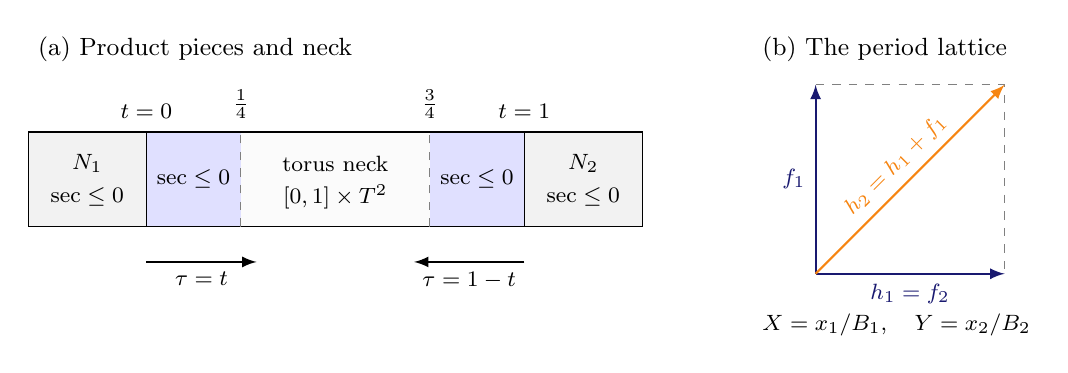
\begin{tikzpicture}[x=1cm,y=1cm,>=latex,font=\footnotesize]
  \node[anchor=west,font=\small] at (0,3.15)
    {(a) Product pieces and neck};
  \fill[gray!10] (0,0.9) rectangle (1.5,2.1);
  \fill[gray!10] (6.3,0.9) rectangle (7.8,2.1);
  \fill[Blue!12] (1.5,0.9) rectangle (2.7,2.1);
  \fill[Blue!12] (5.1,0.9) rectangle (6.3,2.1);
  \fill[gray!3] (2.7,0.9) rectangle (5.1,2.1);
  \draw (0,0.9) rectangle (7.8,2.1);
  \draw (1.5,0.9) -- (1.5,2.1);
  \draw (6.3,0.9) -- (6.3,2.1);
  \draw[dashed,gray] (2.7,0.9) -- (2.7,2.1);
  \draw[dashed,gray] (5.1,0.9) -- (5.1,2.1);
  \node at (0.75,1.7) {$N_1$};
  \node at (7.05,1.7) {$N_2$};
  \node at (0.75,1.28) {$\sec\le0$};
  \node at (7.05,1.28) {$\sec\le0$};
  \node at (2.1,1.5) {$\sec\le0$};
  \node at (5.7,1.5) {$\sec\le0$};
  \node at (3.9,1.7) {torus neck};
  \node at (3.9,1.28) {$[0,1]\times T^2$};
  \node[above] at (1.5,2.15) {$t=0$};
  \node[above] at (2.7,2.15) {$\frac14$};
  \node[above] at (5.1,2.15) {$\frac34$};
  \node[above] at (6.3,2.15) {$t=1$};
  \draw[->,thick] (1.5,0.45) -- (2.9,0.45)
    node[midway,below] {$\tau=t$};
  \draw[->,thick] (6.3,0.45) -- (4.9,0.45)
    node[midway,below] {$\tau=1-t$};

  \node[anchor=west,font=\small] at (9.2,3.15)
    {(b) The period lattice};
  \draw[dashed,gray] (10,2.7) -- (12.4,2.7) -- (12.4,0.3);
  \draw[->,thick,MidnightBlue] (10,0.3) -- (12.4,0.3)
    node[midway,below] {$h_1=f_2$};
  \draw[->,thick,MidnightBlue] (10,0.3) -- (10,2.7)
    node[midway,left] {$f_1$};
  \draw[->,thick,BurntOrange] (10,0.3) -- (12.4,2.7)
    node[midway,above,sloped] {$h_2=h_1+f_1$};
  \node[anchor=west] at (9.2,-0.35)
    {$X=x_1/B_1,\quad Y=x_2/B_2$};
\end{tikzpicture}
\caption{The construction in schematic coordinates.  Each product piece
$N_i$ includes its convex collar; the two end portions of the neck also have
nonpositive sectional curvature.  The arrows indicate the inward
coordinate at each end.  The lattice cell is drawn in normalized
coordinates $(X,Y)$: since $B_1=\epsilon B_2$, its diagonal represents
$h_2=B_2(e_2+\epsilon e_1)=h_1+f_1$ even when the coordinate shear
$\epsilon$ is small.  Physical lengths are not to scale, and drawn angles
are not angles of the Riemannian metric.}
\label{fig:neck-gluing}
\end{figure}

